\chapter{Pruebas y Resultados} \label{chap:resultadosExperimentales}

Este capítulo se centra en análisis de las pruebas realizadas para evaluar la efectividad y eficiencia del sistema desarrollado. Estas pruebas se clasifican en tres categorías principales. Cada una de estas pruebas juega un papel crucial en la validación del sistema, asegurando que cumple con los requisitos establecidos y proporciona una experiencia de usuario satisfactoria. Los resultados obtenidos no solo demuestran la viabilidad del sistema, sino que también ofrecen \textit{insights} valiosos para futuras mejoras y ajustes.

\section{Pruebas de Funcionalidad}

Esta sección se centra en las diferentes pruebas de funcionalidad realizadas para garantizar la calidad y el correcto funcionamiento del sistema. Estas pruebas incluyen diferentes tipos de prueba, ya que cada una de ellas dirigida a validar aspectos específicos de la plataforma.

\subsection{Pruebas Unitarias}

Las pruebas unitarias se enfocaron en validar la funcionalidad de los componentes individuales del sistema. Concretamente, se escribieron casos de prueba para cada función y método, cubriendo tanto los escenarios esperados como los casos extremos. Se validaron las salidas de cada componente para garantizar que cumplieran con las especificaciones y requisitos funcionales. Se prestó especial atención a la cobertura de código, buscando lograr un porcentaje alto que garantice la fiabilidad del sistema.

\subsection{Pruebas de Integración}

Las pruebas de integración se centraron en la interacción entre los componentes individuales del sistema para asegurar que funcionaran juntos de manera efectiva.

Se probaron las interfaces y las interacciones entre diferentes módulos y servicios. Se realizaron pruebas de llamadas a APIs, interacción con bases de datos y comunicación entre servicios. Se identificaron y corrigieron problemas de integración, como incompatibilidades y fallos en la transferencia de datos con la ayuda de Postman \cite{postman}. 

\subsection{Pruebas Manuales}
Las pruebas manuales fueron cruciales para validar la experiencia del usuario y la funcionalidad desde una perspectiva más humana. Se llevaron a cabo sesiones de prueba donde se interactuaba con la aplicación de manera natural, buscando errores o problemas de usabilidad. Se observó el comportamiento de la aplicación en diferentes dispositivos y sistemas operativos para asegurar su compatibilidad y adaptabilidad. Se realizaron pruebas de escenarios de usuario, simulando diferentes flujos de trabajo y operaciones comunes.

\subsection{Pruebas de Navegación y Flujo de Usuario}

Estas pruebas se enfocaron en la experiencia del usuario al navegar por la aplicación y realizar tareas específicas, asegurando una interfaz intuitiva y eficiente. Se evaluó la lógica y coherencia de la interfaz de usuario, asegurando que los flujos de trabajo fueran claros y fáciles de seguir. Se prestó atención a la experiencia del usuario al completar tareas comunes, buscando minimizar la complejidad y maximizar la eficiencia.

En resumen, las pruebas de funcionalidad jugaron un papel fundamental en la validación y mejora continua del sistema, asegurando que cumpliera con los requisitos funcionales y proporcionara una experiencia de usuario satisfactoria antes de la prueba con niños.


\section{Pruebas de Rendimiento}

Las pruebas de rendimiento se llevaron a cabo para evaluar la capacidad del sistema para manejar cargas de trabajo significativas y para identificar cualquier posible cuello de botella. Se utilizaron escenarios de prueba que reflejaban el uso típico del sistema por parte de los usuarios finales.

Se empleó Apache JMeter \cite{jmeter}, una herramienta de prueba de carga de código abierto, para simular múltiples solicitudes al servidor, con el fin de imitar el comportamiento de varios usuarios accediendo al sistema simultáneamente. 

La configuración de JMeter se ajustó para incrementar gradualmente el número de usuarios virtuales y generar una carga significativa en el servidor.

\subsection{Configuración de la Prueba}

La configuración de la prueba incluyó:

\begin{itemize}
    \item Número total de peticiones: 10,000
    \item Usuarios concurrentes (hilos): 1,000
    \item Duración de la prueba: 10 minutos
    \item Tiempo de rampa: 100 segundos
\end{itemize}

\subsection{Resultados Observados}

Los resultados de las pruebas mostraron que el sistema era capaz de manejar un throughput de 96.92 peticiones por minuto con una variabilidad en los tiempos de respuesta. Los tiempos de respuesta promedio se mantuvieron en 44 ms, con una mediana de 12 ms, lo que indica una respuesta rápida bajo carga para la mayoría de los usuarios.

\begin{figure}[H]
\centering
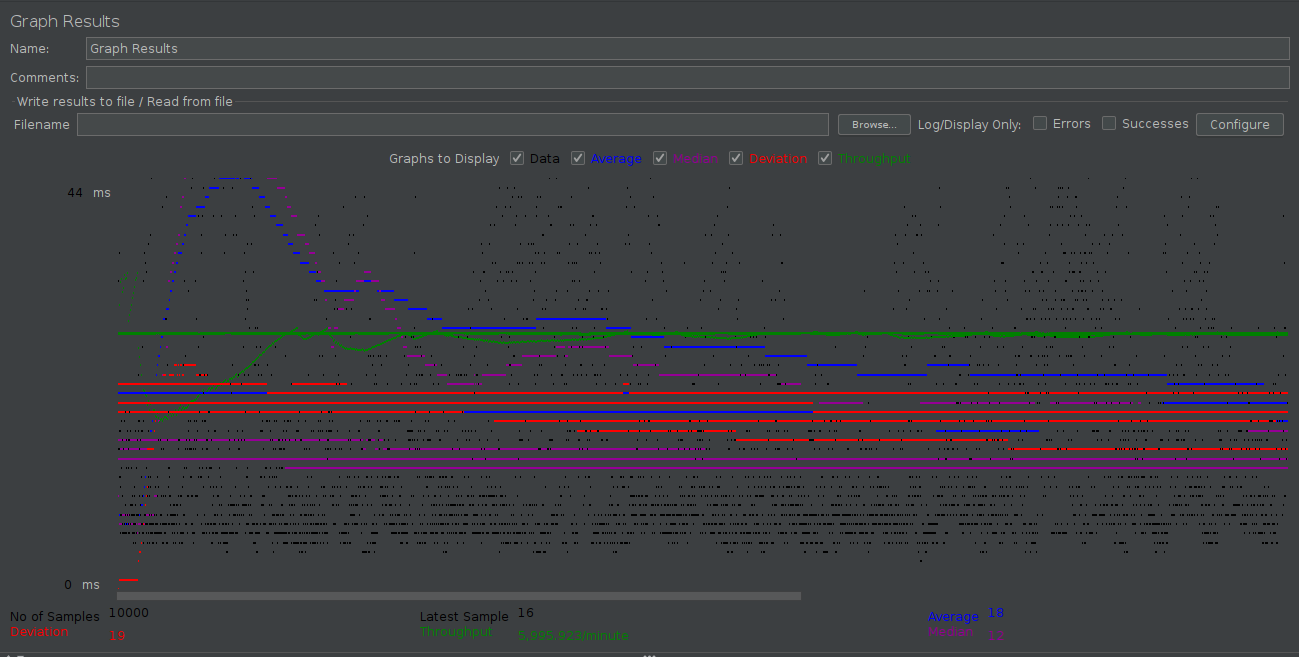
\includegraphics[width=\textwidth]{imagenes/graforendimiento.png}
\caption{Resultados gráficos de la prueba de rendimiento con JMeter.}
\label{fig:grafico-jmeter}
\end{figure}

Los datos recogidos sugieren que la experiencia del usuario se mantendría consistente hasta cierto punto de carga. Sin embargo, se observaron advertencias relacionadas con la gestión de cookies, lo que podría ser un indicador de problemas de configuración en el manejo de sesiones de usuario o en el estado del sistema.

El análisis de los resultados recogidos sugiere que el sistema es robusto y puede manejar cargas de usuarios concurrentes de manera efectiva hasta un punto crítico. Cumpliendo, de esta manera, el requisito \ref{table:req-RNF38} del tiempo de respuesta establecido en la fase de análisis del proyecto.

\section{Pruebas de Usabilidad}

Con el fin de evaluar correctamente el sistema implementado, también se realizaron pruebas con un pequeño pero significativo grupo de niños, compuesto por 3 participantes de distintas edades. Concretamente de 8, 12 y 15 años. Cada uno de ellos interactuó con el sistema de manera individual, en sesiones separadas. De esta manera, se obtuvo una evaluación más detallada y precisa de la eficacia del sistema.

Las tareas asignadas para las pruebas en la página web incluyeron (véase anexo \ref{chap:guion}):

\begin{itemize}
    \item Navegación por el sitio y localización de información específica.
    \item Resolución de ejercicios de programación y lógica.
    \item Cuestionario oral sobre la lectura de contenidos de teoría o enunciados de ejercicios.
\end{itemize}

Los indicadores cuantitativos mostraron resultados bastante alentadores. Se registró el tiempo en la tabla \ref{tab:pruebast} donde se puede visualizar el tiempo que cada participante empleó en completar las tareas asignadas:

\begin{table}[h]
\centering
\begin{tabular}{|c|c|c|c|}
\hline
Edad   & Navegación (min) & Ejercicios (min) & Cuestionario (min) \\ \hline
8 años & 14              & 23               & 22                 \\ \hline
12 años & 10              & 15               & 12                 \\ \hline
15 años & 6               & 14              & 10                 \\ \hline
\end{tabular}
\caption{Tiempo empleado en tareas por edad}
\label{tab:pruebast}
\end{table}

Los jóvenes usuarios lograron completar los ejercicios con éxito. Además, el tiempo que pasaron interactuando con la plataforma se mantuvo en un rango óptimo. Por lo tanto, se puede decir que el sistema fue eficaz en adaptarse a la dificultad. Sin embargo, se observó que el tiempo óptimo de interacción con el sistema debería ajustarse según la edad del usuario, dado que las capacidades de atención y ritmo de lectura varían considerablemente en función de la edad. 

En términos de usabilidad, las respuestas fueron positivas. La plataforma fue calificada como fácil de usar y práctica, lo cual indica que el diseño de la interfaz es adecuado. La claridad en las instrucciones también fue un punto destacado aunque a veces desconcertante para los más pequeños debido a su capacidad de distracción.

Entre las sugerencias aportadas, la más recurrente fue la adición de elementos como juegos con tal de incrementar la motivación y el compromiso. Este tipo de retroalimentación fue especialmente valiosa y se consideró como una mejora importante a realizar en el sistema. Además, la metodología de pruebas individuales permitió recoger opiniones y sugerencias sin la influencia o presión del grupo.

En conclusión, las pruebas iniciales sugirieron que el sistema era efectivo en su misión de ofrecer una experiencia de aprendizaje adaptativo. Los comentarios y observaciones de los jóvenes participantes ofrecieron un conjunto invaluable de datos que sirvieron para enriquecer el sistema.
